\documentclass{article}
\usepackage[utf8]{inputenc}
\usepackage{geometry}
\usepackage{graphicx}
\usepackage{float}
\geometry{legalpaper, portrait, margin=1.5in}
\usepackage{amsmath}
\title{%
	A Markowitz Portfolio Optimiser \\
	\large Computational Finance with C++ \\}
\author{CID: 01805027}
\date{10 June 2020}
\usepackage[thinc]{esdiff}
\usepackage{hyperref}
\usepackage{algorithm} 
\usepackage{algpseudocode} 
\usepackage{listings}
\usepackage{color}

\definecolor{dkgreen}{rgb}{0,0.6,0}
\definecolor{gray}{rgb}{0.5,0.5,0.5}
\definecolor{mauve}{rgb}{0.58,0,0.82}

\lstset{frame=tb,
	language=C++,
	aboveskip=3mm,
	belowskip=3mm,
	showstringspaces=false,
	columns=flexible,
	basicstyle={\small\ttfamily},
	numbers=none,
	numberstyle=\tiny\color{gray},
	keywordstyle=\color{blue},
	commentstyle=\color{dkgreen},
	stringstyle=\color{mauve},
	breaklines=true,
	breakatwhitespace=true,
	tabsize=3
}


\begin{document}
	
%\tableofcontents
	
	
\renewcommand*{\arraystretch}{1.5}

\maketitle
\section{Introduction} 
\label{sec:introduction}

Since their inception, economists, mathematicians, physicists and computer scientists the like have sought to 'beat' the markets by employing novel developments in their respective fields.

One such forum in which attempts have been made is the problem of portfolio choice. It is widely accepted that a goal of investing in financial markets is to make as much excess return as possible for a given level of risk taken on (idiosyncratic and non-idiosyncratic). 

This is characterised well by the Efficient Frontier as seen in Figure (\ref{fig:efficient_frontier}).


\begin{figure}[H]
	\centerline{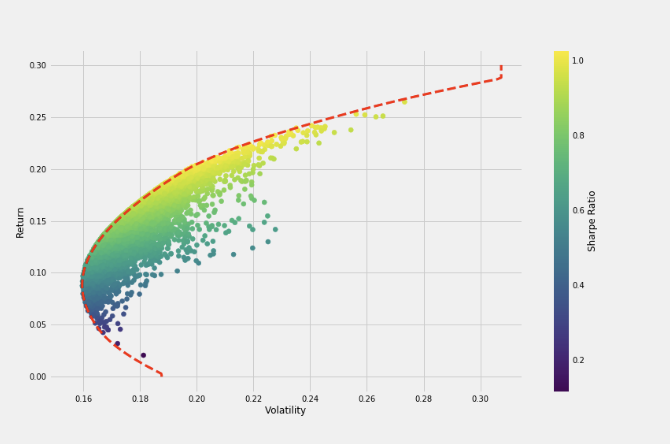
\includegraphics[width=\textwidth,height=4in]{figures/EF.png}}
	\caption{Expected return against volatility. The red dashed line characterises the efficient frontier itself, on which the optimal portfolios lie. \cite{ef_medium} Note here the term \textit{volatility} is used to represent the variance of the portfolios, not the standard deviation as is traditional.}
		\label{fig:efficient_frontier}
\end{figure}


Optimal portfolios lie on the dashed red line, named the \textit{Efficient Frontier} as it characterises the portfolios that make as much excess return as possible for a given risk appetite, denoted by its position along the horizontal axis. The points in the centre of the concave function are examples of suboptimal portfolios. These portfolios carry more risk than the theory requires for their level of expected excess return, or similarly do not return enough above the risk free rate for the amount of risk they take on.

No portfolios exist outside of the frontier since this scope corresponds to portfolios that achieve a theoretically impossibly large return for a given risk appetite, or conversely  and impossibly small level of risk for a quoted level of remuneration.


It must be noted that mean-variance efficiency is a corner-stone of modern portfolio choice theory, even appearing as an assumption to the renowned Capital Asset Pricing Model (CAPM) \cite{capm}; it is assumed that 'all market participants are mean-variance efficient optimisers'. Though the subtle but important point must be made that the CAPM states that all market participants are rewarded for the amount of \textit{non-diversifiable, systematic risk} taken on, and says there shall be no remuneration for \textit{diversifiable, idiosyncratic risks} which are generally included in the measures of portfolio volatility used for the efficient frontier plot above.


As a result, this project seeks to solve the portfolio choice problem by an implementation of Markowitz Portfolio Theory \cite{mpt} in C++ using the Quadratic Conjugate Method and a backtesting framework to test the resulting portfolio.



\subsection{Theory}
\label{sec:theory}

The formal mathematical derivation below largely following notes provided by Parpas, P \cite{notes} are included for the context of the problem.

We define a target return, $\overline{r_p}$, for the portfolio and wish for it to return this level of compensation for as little risk (portfolio variance) as possible. 

Therefore a system of Lagrange multipliers are used to define the constraints and requirements on the portfolio. Namely, to:


\begin{enumerate}
	\item \textbf{Minimise portfolio variance, $\sigma_p^2$}  - Equation (\ref{eqn:portfolio_variance}).

	\item \textbf{Ensure the expected portfolio return is equal to the target return, $\overline{r_p}$} - Equation (\ref{eqn:target_return_constraint}).
	
	\item \textbf{Constrain the allocation of funds} - to ensure that the portfolio does not see an over or under-allocation of the funds available to it; it must have invested all resources available to it at any time - Equation (\ref{eqn:weights_constraint}).
	
\end{enumerate}

Note that there have been no constraints placed on the individual values of the portfolio weight of asset $i$, $w_i$. In other similar studies \cite{mpt} constraints such as ensuring the positivity of $w_i$ are employed to forbid the system from short selling a security. This constraint has not been imposed here; the model is freely able to short sell a security should it see fit.

In Equation (\ref{eqn:portfolio_variance}), we define the variance of the Markowitz portfolio, $\sigma_{p}^{2}$, with a preceding factor of $\frac{1}{2}$ for convenience. $\sigma_{ij}$ is the covariance between stocks $i$ and $j$.


\begin{equation}
\dfrac{1}{2} \sigma^{2}_{p} =  \dfrac{1}{2} \sum_{i,j=1}^{n} w_{i} \sigma_{ij} w_{j}
\label{eqn:portfolio_variance}
\end{equation}

The variance of the portfolio is minimised via the Lagrange method in line with point 1 above, while ensuring the following two constraints are also upheld:

\begin{equation}
\sum_{i=1}^{n} w_{i} \overline{r_i} - \overline{r_p} = 0
\label{eqn:target_return_constraint}
\end{equation}

Above, we mandate that the portfolio return is equal to the value target return $\overline{r_p}$ in line with point 2 above. By setting $\overline{r_p}$, we have effectively chosen the portfolio return we desire and thus the weights the optimisation method yields.

Below in Equation (\ref{eqn:weights_constraint}) is the constraint on the sum of the portfolio weights equalling unity. This ensures that the portfolio does not over or under-allocate the funds available to it in line with point 3 above.

\begin{equation} 
\sum_{i=1}^{n} w_{i} - 1 = 0
\label{eqn:weights_constraint}
\end{equation}

\begin{equation} 
L(w, \lambda, \mu) =  \dfrac{1}{2} \sum_{i,j=1}^{n} w_{i} \sigma_{ij} w_{j} 
	-\lambda \left( \sum_{i=1}^{n} w_{i} \overline{r_i} - \overline{r_p}) \right)
	- \mu \left( \sum_{i=1}^{n} w_{i} - 1 \right)
\label{lagrangian}
\end{equation}

Finally, Equation(\ref{lagrangian}) shows the Lagrangian we seek to minimise, with $\lambda$ and $\mu$ the Lagrange multipliers for each of the constraints Equation (\ref{eqn:target_return_constraint}) and Equation (\ref{eqn:weights_constraint}).

For convenience when scaling to a large number of assets and to code in the possibility of introducing further constraints, we introduce the following matrix notation:

\begin{description}
\item [$\bullet$ $\emph{w} = (w_1,..., w_n)' \in \Re^n$ ] - a column vector of $n$ portfolio weights for $n$ assets
\item [$\bullet$ $\overline{\emph{r}} = (\overline{r_1},..., \overline{r_n})' \in \Re^n$ ] - a column vector of expected asset returns
\item [$\bullet$ $\emph{e} = (1,..., 1)' \in \Re^n$ ] - the unit column vector of length $n$
\item [$\bullet$ $\emph{0} = (0,..., 0)' \in \Re^n$ ] - the zero column vector of length $n$
\end{description}

The Lagrangian in matrix form is shown below in Equation (\ref{vector_lagrangrian}) where $\Sigma \in \Re^{n \times n}$ is the covariance matrix of the assets. Explicitly, $\Sigma_{ij}$ is the ${ij}^{th}$ element of the matrix which is equal to the (scalar) value of the covariance between asset $i$ and $j$,  $\sigma_{ij}$.

\begin{equation} 
L(\textbf{w}, \lambda, \mu)  = \dfrac{1}{2} \textbf{w}'\Sigma\textbf{w}
-\lambda \left( \textbf{w}'\overline{\textbf{r}} - \overline{r_p}\right)
-\mu \left( \textbf{w}'\textbf{e} - 1\right)
\label{vector_lagrangrian}
\end{equation}

Now, in order to minimise the Lagrangian it must be differentiated with respect to the weights, {\textbf{w}}. Finding the rate of change of the system's Lagrangian with respect to the portfolio weights and setting the resulting equation to zero will yeild the turning point of the function in weights-space.

\begin{equation}
\diff{L(\textbf{w}, \lambda, \mu)}{\textbf{w}'} =  \Sigma\textbf{w}
-\lambda \overline{\textbf{r}}
-\mu\textbf{e} = 0
\label{eqn:optimality_lagrangian}
\end{equation}

It may be seen by inspection that the second derivative of the Lagrangian with respect to $\textbf{w}$  is indeed positive for all values of $\textbf{w}$, implying that this is indeed a minimum and that the function itself is concave. Note that this is aligned with our expectation that the efficient frontier is concave, as in Figure (\ref{fig:efficient_frontier}).

With Equations (\ref{eqn:target_return_constraint}) and (\ref{eqn:weights_constraint}) also required for optimality, we may write the system of $n+2$ simultaneous equations as a single matrix equation written in the form $Ax = b$, below in Equation (\ref{matrix_eqn}). where $A \in \Re^{(n+2) \times (n+2)}$ and $x,\; b \in \Re^n$. We seek to solve Equation (\ref{matrix_solved}) numerically via the Quadratic Conjugate Method to find the vector of weights $w$ that yield the desired portfolio return, $\overline{r_p}$.

\begin{equation}
\begin{bmatrix}
\Sigma & -\overline{\textbf{r}} & -\textbf{e} \\
-\overline{\textbf{r}}'  & 0 & 0 \\
-\textbf{e}' & 0 & 0 
\end{bmatrix}
\begin{bmatrix}
\textbf{w}\\
\lambda \\
\mu
\end{bmatrix}
=
\begin{bmatrix}
\textbf{0}\\
-\overline{r_p}\\
-1
\end{bmatrix}
\label{matrix_eqn}
\end{equation}


\begin{equation}
\begin{bmatrix}
\textbf{w}\\
\lambda \\
\mu
\end{bmatrix}
=
\begin{bmatrix}
\Sigma & -\overline{\textbf{r}} & -\textbf{e} \\
-\overline{\textbf{r}}'  & 0 & 0 \\
-\textbf{e}' & 0 & 0 
\end{bmatrix}^{-1}
\begin{bmatrix}
\textbf{0}\\
-\overline{r_p}\\
-1
\end{bmatrix}
\label{matrix_solved}
\end{equation}


\section{Implementation}
\label{sec:implementation}



We test the portfolio composed of assets weighted by the weights forming the solution of Equation (\ref{matrix_solved}). This is done for 83 of the FTSE 100 assets over a period of 700 days in total. Each in sample window is 100 days long, used to calibrate the weights to generate a portfolio with the lowest viable risk exposure for a predetermined target portfolio return: $\overline{r_p}$. 


\begin{figure}[H]
	\centerline{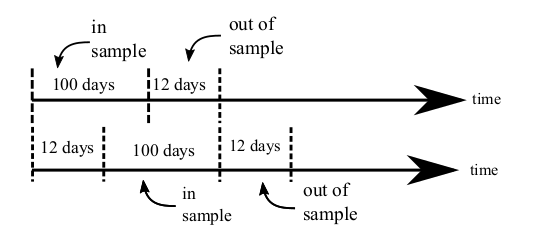
\includegraphics[width=3.5in,height=1.5in]{figures/backtesting_windows.png}}
	\label{backtetsing_window}
	\caption{Organisation of the rolling balancing and backtesting windows. \cite{assignment}}
\end{figure}

More precisely, for day $t_i$ with $i$ in the following ranges, the backtest is in the corresponding balancing or evaluation phase:  

\begin{description}
	\item [$\bullet$ In sample (balance) window 1] - $t_i\:\forall\:i\:\in [0,99]$
	\item [$\bullet$ Out of sample (evaluation) window 1] - $t_i\:\forall\:i\:\in [100,111]$
	\item [$\bullet$ In sample(balance) window 2] - $t_i\:\forall\:i\:\in [12, 111]$
	\item [$\bullet$ Out of sample (evaluation) window 2] - $t_i\:\forall\:i\:\in [112, 123]$
\end{description}

This continues until the end of the 700 day dataset is reached. In total, the application balances 50 times, generates 50 new sets of weights, and evaluates these 50 times for each target return.


\subsection{Code}
\label{sec:implementation_code}


With a distinct focus on code readability, maintainability and efficiency, the backtesting frameworks, Quadratic Conjugate Method and other necessary tools for the Markowitz optimised portfolio were written in C++ (which may be seen explicitly in the or in the \href{https://github.com/indipanesar96/markowitzportfoliooptimiser}{public repository} or in the source files included in the submission).


The project code was split into five distinct project directories for the easy of maintenance and cleanliness. The directories and their contents are outlined briefly in the following sections.



\subsubsection{Utility}
\label{sec:utility}

The Utility contains the classes and headers for \textit{VectorUtil, Matrix, RunConfig} and struct \textit{BacktestResults}. The first two housed small building-block-esque functions upon which the entirety of the application is based. As such, it was vital that these methods used to perform arithmetic operations on the rank 1 and 2 tensors were well tested and efficient. Here and in general throughout the application, objects were passed to one another by pointer if possible to avoid the unnecessary duplication of items in memory.

Creating these classes first greatly increased the speed and accuracy of development of the more complex classes that followed.
It was imperative that the arithmetic functions in \textit{VectorUtil.h} were as generic as possible. As a result, generic types were used throughout, though a condition was imposed in the typename signature that ensured the types being passed were numeric, as can be seen in the snippet below:


\begin{lstlisting}
// VectorUtil.h

template<typename T,
	typename = typename enable_if< is_arithmetic<T>::value, T> ::type>
vector<T> vectorLinearCombination(T aCoeff, vector<T> *a, T bCoeff, vector<T> *b) 
{
	int aSize = a->size();
	int bSize = b->size();
	if (aSize != bSize) {
		cout << "Vectors aren't the same size and so cannot be subtracted/added from/to one another." << endl;
		cout << "\t Sizes: " << aSize << " and " << bSize;
		exit(12);
	}
	
	vector<double> result = vector<double>(aSize);
	for (int i = 0; i < aSize; i++) {
		result[i] = aCoeff * a->at(i) + bCoeff* b->at(i);
	}

	return result;
}
\end{lstlisting}

Also seen in the above method is the helpful error message and an easily searchable error code when it receives data incompatible with the operation, for ease of debugging.

\textit{RunConfig} is a data class used to group pieces of information in a convenient manor also requiring a method on the object; \textit{RunConfig::setNAssets()} is used to change the number of assets taken into account for the time complexity analysis discussed later. It contained parameters that were pertinent to a particular run of the backtest. It was useful to run the application on small and medium sized subsets of the data for debugging purposes and so with each of these came a set of parameters (in/out of sample window lengths, for example) that were specific to the dataset in question. It became cleaner and more convenient to group these parameters together into one object (a \textit{RunConfig} object) and pass this to \textit{Portfolio::backtest()}.  

I found this line of reasoning around ease of use to be especially pertinent with method signatures since their readability contributes massively to the readability of the application as a whole.  

The \textit{BacktestResults} struct was useful in combining mutually relevant results; the mean realised portfolio return and variance in and out of sample. Further, it acted as a safety measure as it allowed the strong typing of variables of type double, preventing errors associated with accessing the wrong one. For example, \textit{BacktestResults.retOOS} irrefutably returned the out of sample return. Had these four doubles been placed into a list, the user at the callsite would have to have prerequisuite knowledge of the indices of the list (for example knowing that out of sample return would be the 3rd element in the list) - a practice prone to well disguised bugs.

\subsubsection{Repository}
\label{sec:repository}

Repository houses the classes and methods used to load data in from the comma separated value files. The functionality here was mostly provided with few other editions required. One such edition made was the ability to only read in from disk the number of columns required, dictated by \textit{RunConfig.nAssets}.


\subsubsection{Estimator}
\label{sec:parameter_estimation}

This directory holds the \textit{ParamaterEstimator} class and its header, a prime example for the use case of a singleton object design pattern. The class holds public static methods that calculate various parameters such as the means, covariances and standard deviations of the aforementioned vector and self-made Matrix objects passed to it. It maintains no state and has no attributes; testament to the functional approach to programming commonly used when encoding mathematical functions.

As these functions were to be called many times through the one backtest, their efficiency was paramount. An example of this is the \textit{ParamaterEstimator::estimateCovariances()} method capitalising on the symmetry property of the covariance matrix. Specifically, the index over the second dimension only ran up from zero to the value of the first index, resulting in only one of the upper or lower triangular portions of the matrix being computed before the result is assigned to two symmetrical element locations.

\begin{lstlisting}
// ParameterEstimator.cpp

Matrix ParameterEstimator::estimateCovariances 
	(Matrix *m, vector<double> *meanReturns) {

	int nAssets = m->getNCols();
	int nDays = m->getNRows();
	
	Matrix covariances = Matrix(nAssets, nAssets);
	
	for (int a1 = 0; a1 < nAssets; a1++) {
		double a1mean = meanReturns->at(a1);
		// only calculating values for the lower triangle of the matrix and
		// using the fact that it's symmetric
		for (int a2 = 0; a2 <= a1; a2++) {
			double a2mean = meanReturns->at(a2);
			double temp = 0.0;
	
			for (int day = 0; day < nDays; day++) {
				temp += (m->get(day, a1) - a1mean) * (m->get(day, a2) - a2mean);
			}
			
			//assigning to symmetric elements simultanously
			covariances.set(a1, a2, (temp / (nDays - 1)));
			covariances.set(a2, a1, (temp / (nDays - 1))); 
		}
	}
	
	return covariances;
}
\end{lstlisting}


\subsubsection{Optimiser}
\label{sec:portfolio_optimiser}

The \textit{PortfolioOptimiser} class and header are held in this directory and are where the Quadratic Conjugate Method is implemented. It was necessary for this class to maintain a state, having attributes on it that would be required across multiple of its methods. These attributes consisted of constant parameters from the \textit{RunConfig} of the current simulation, such as the initial values for the Lagrange multipliers $\lambda$ and $\mu$ and the tolerance to which we declare the optimisation method as having converged. 

It was found after some experimentation that the initial values of $\lambda$ and $\mu$ had little effect on the evolution of the alogorithm, understandably so, since it is solving a linear set of equations.

In addition, a getter and setter are employed to set the target return for the optimiser, $\overline{r_p}$ as the same instance of the \textit{PortfolioOptimiser} is used to solve for all different target returns.



\subsubsection{Backtest}
\label{sec:backtestcode}

The Backtest directory is where the \textit{Portfolio} class, header and \textit{main.cpp} are situated. The \textit{main.cpp} acts as the entry point into the application; where the \textit{RunConfigs} were initialised and sent to the aforementioned \textit{Portfolio::backtest()} method.

Inside its constructor, \textit{Portfolio::Portfolio()}, the returns data required for the backtest is loaded from disk into a Matrix object using the tools in \textit{DataRepository}.

From \textit{main.cpp}, \textit{Portfolio::backtest()} is called, the target return for this run is set and the days are iterated through. The returns matrix is spliced using the day numbers as indices; their values corresponding to the appropriate balancing and evaluating windows as described above in section \ref{sec:implementation}.

For each window, the balancing window's matrix of (in sample) returns is passed by pointer to the \textit{PortfolioOptimiser::calculateWeights()} which in turn calls a series of its own helper functions to return the weights. 

Once received, \textit{Portfolio::checkWeights()} is called to ensure the sum of the weights is to within a predefined tolerance of unity (tolerance defined in \textit{RunConfig}). This is vital, if the check fails the application is exited with a debug line and an error code. 

The weights are then passed with the test window's matrix (out of sample) to \textit{Portfolio::evaluate()} to evauluate the return of the portfolio over the out of sample window. The same weights are also passed with the in sample matrix of returns, generating the in sample returns for comparison.


These steos are repeaated for as many balancing and evaluating windows there are (50 in this dataset) while the key metrics; portfolio returns and variance are stored for comparison with runs of different target returns.


We now move to a more detailed discussion of the calculation of the weights themselves as the solution to Equation (\ref{matrix_solved}) by the Quadratic Conjugate Method.


\subsection{Quadratic Conjugate Method}
\label{sec:qcm}


Recall that the Markowitz Portfolio Choice Problem was reduced to a matrix equation of the form $Ax = b$ and that the Quadratic Conjugate Method solves this for vector $x$ numerically, with $x$ defined as:


\begin{equation}
x=
\begin{bmatrix}
\textbf{w}\\
\lambda \\
\mu
\end{bmatrix}
\end{equation}

An initialisation of $x_0$ is required for the method and so the weights \textbf{w} are chosen such that the initial portfolio is equally weighted (with a portfolio of $n = 83$ assets this is equivocates to setting all $w_i \approx 0.01205$). Inital values for the Lagrange multipliers $\lambda$ and $\mu$ are set to 0.5 each though it was discovered that the initialisation of the two multipliers has little to no effect on the subsequent optimisation results. This is understandable since the method is used to solve a linear set of equations. It can therefore be expected that the starting points of parameters are inconsequential as linear systems do not have local minima for the algorithm to become trapped in when searching for a solution.

A value of $\epsilon$ is required as our tolerance limit whereby convergence of the algorithm is defined when the modulus of the error term $s_{k+1}$ squared is less than $\epsilon$. This value is passed through to the private \textit{PortfolioOptimiser::conjugateGradientMethod()} from the $RunConfig$ and a suitable value was found to be $10^{-6}$.

\begin{algorithm}[H]
	\caption{Quadratic Conjugate Method} 
	
	Initialization: $k=0, s_0 \equiv b - Ax_0, p_0 \equiv s_0$;
	
	\begin{algorithmic}[1]
		\While {$s_{k}'s_{k} > \epsilon$}
		\State $\alpha_k = \frac{s_{k}'s_{k}}{p_{k}'Ap_{k}}$
		\State $x_{k+1} = x_{k} + 	\alpha_kp_{k}$
		\State $s_{k+1} = s_{k} - 	\alpha_kAp_{k}$
		\If{$s_{k+1}'s_{k+1} < \epsilon$}
		\State exit
		\EndIf
		\State $\beta_k = \frac{s_{k+1}'s_{k+1}}{s_{k}'s_{k}}$
		\State $p_{k+1} = s_{k+1} - 	\beta_kp_{k}$
		\State $k+=1$
		\EndWhile 
		
		
		you may like to fix their values at the beginning.
		
		Notice that you should not get (very) different results for different initialization values.
		
		At the end of the day, this is a method that gives you the solution of a linear system!
	\end{algorithmic} 
\end{algorithm}


Though it must be noted that varying $\epsilon$ by a factor of $10^2$ smaller or larger seemed to have no effect on the rate of convergence. After some further investigation it was found that for the numbers typical to this context, the product $s_{k}'s_{k}$ jumps discontinuously from around $10^{-3}$ to $10^{-10}$. More generally, convergence has been proven to occur in fewer than iterations than the number of rows in matrix $A$ \cite{qcm_convergence}. This implies convergence is guaranteed in fewer than $n+2$ iterations, 85, in this dataset.


All variables apart from the result, $x_{k+1}$ are discarded when the thread leaves the scope as they are no longer required. Finally, the weights $w_{i}$ are retrieved from the first $n$ elements of $x_{k+1}$ and passed back to \textit{Portfolio::backtest()} to be evaluated on our of sample test window. 




\section{Results \& Discussion}
\label{sec:results}


As this is an exercise in implementing a numerical optimisation method to financial data, the results of the application are judged by its adherance to the constraints imposed by the theory in \hyperref[sec:theory]{section 1.1}.

The success of the application will, in part, be measured by its ability to generate weights that form a portfolio yielding the target return specified \textit{in sample}. Should it be successful in achieving this, then it may be said that the application is successful in its implementation of the Quadratic Conjugate Method. 



More precisely, there are two factors at play in this investigation: 


\begin{enumerate}
	\item \textbf{the implementation of the Quadratic Conjugate Method} - and its success or failure in generating weights that satisfy Equation (\ref{matrix_solved}) \textit{in sample}.
	
	\item \textbf{the Markowitz approach to portfolio choice optimisation} - and its success or failure in generating a portfolio that yields a specified target return \textit{out of sample}.
		
\end{enumerate}


The success of the former shall be verified by the ability of the portfolio to produce the target return \textit{in sample}.

The latter's succes shall be verified by the ability of the portfolio to produce the target return \textit{out of sample}.


Yielding a portfolio that mimics the target return in sample but not out of sample highlights a flaw with the Markowitz portfolio choice approach itself. Since in this case the Markowitz framework received the weights it required (accurately) as shown by the in sample performance, it may be deduced that any lack of adherance to the target returns by the portfolio out of sample may be solely attributed to shortcomings of the Markowitz appoach itself, not the Quadratic Conjugate Method or its implementation.

Interestingly however, if weights are generated such that the resulting portfolio \textit{does not} yield the target return in sample, no comment can be made on the success or failure of point 2 above, the validity of the Markowitz approach. This is because the ability to test the Markowitz approach in earnest is predicated on the ability to accurately generate the required weights $\textbf{w}$ to specification.


\subsection{Target Return Accuracy}


In sample, the Quadratic Conjugate Method generates weights that yield a portfolio with precisely the target return required (columns one and two of Table \ref{table:port_results}). The variance in these returns was calculated across the 50 test windows per target and are plotted as the error bars. 

Out of sample, we see that the same weights form a portfolio that does not yield the target return in the 12 day (testing) window directly following the 100 day in sample (balancing) window that was used to generate them. This is a clear failing of the Markowitz approach to portfolio choice. 


The success of the Markowitz approach is predicated on the ability predict future returns given the knowledge of past returns. This touches on the question of the existence of the martingality property of underlying stock price dynamics, closely tied to the Efficient Markets Hypothesis (EMH) \cite{martingale}. 

The strongest form of EMH suggests that market efficiency ensures that security prices encode all public and private information at any given point in time. If this is the case, no form of technical analysis, including the Markowitz approach, may be used to generate excess returns consistently. There is some empirical evidence proving that EMH does hold in the markets, such as price movement after earnigns announcements. 

Conversely, the notion that investors are not able to find and capitalise on undervalued assets is flawed. Though since it often requires deep contextual knowledge of the company, leaning more toward fundamental analysis, this line of reasoning is not relevant in this investigation when employing a purely analytical, algorithmic approach to portfolio choice.





\begin{figure}[H]
	\centerline{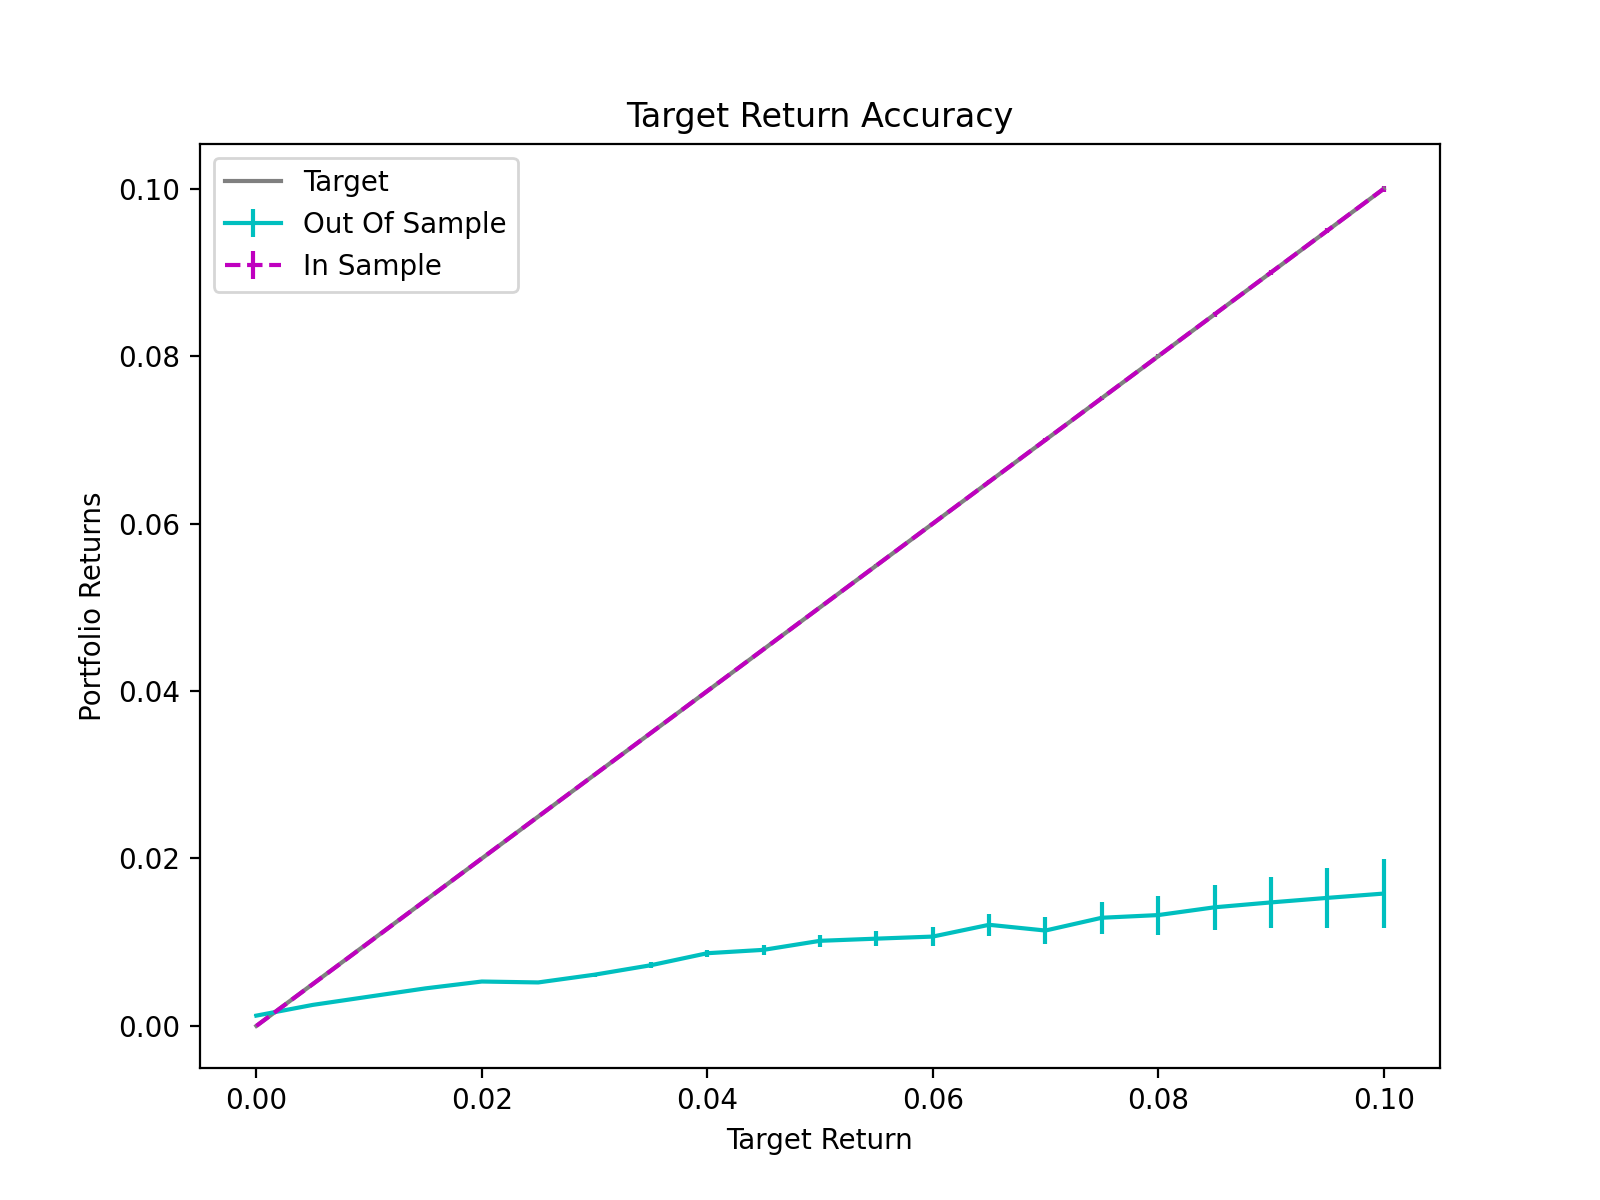
\includegraphics[width=\textwidth]{figures/oos_accuracy.png}}
	\caption{In and out of sample performance of the application in generating a portfolio with the targeted return, the exogenous variable here. Error bars are the variance in the portfolio return. They do not start at the same point as the generated portfolio failed to produce the target return of 0\% for the first data point as seen in Table \ref{table:port_results} of the Appendix (all underlying data is shown).}
	\label{fig:oos_accuracy}
\end{figure}

Using the limited cross-sectional returns data to generate a portfolio with a specified return was naively optimistic at best. The approach of keeping the weights generated in the 100 day balance period constant over the following 12 day test period assumed that the underlying dynamics and dividends issuances of all the securities remained unchanged. Given the timescales in question, this is not inherently a flawed assumption and so one may feasibly expect it to hold. Indeed  Figure \ref{fig:oos_accuracy} could be interpreted as supporting this assumption - as the target return increases so does the realised portfolio return, though just not as much as is required for the Markowitz approach to be validated.




\begin{figure}[H]
	\centerline{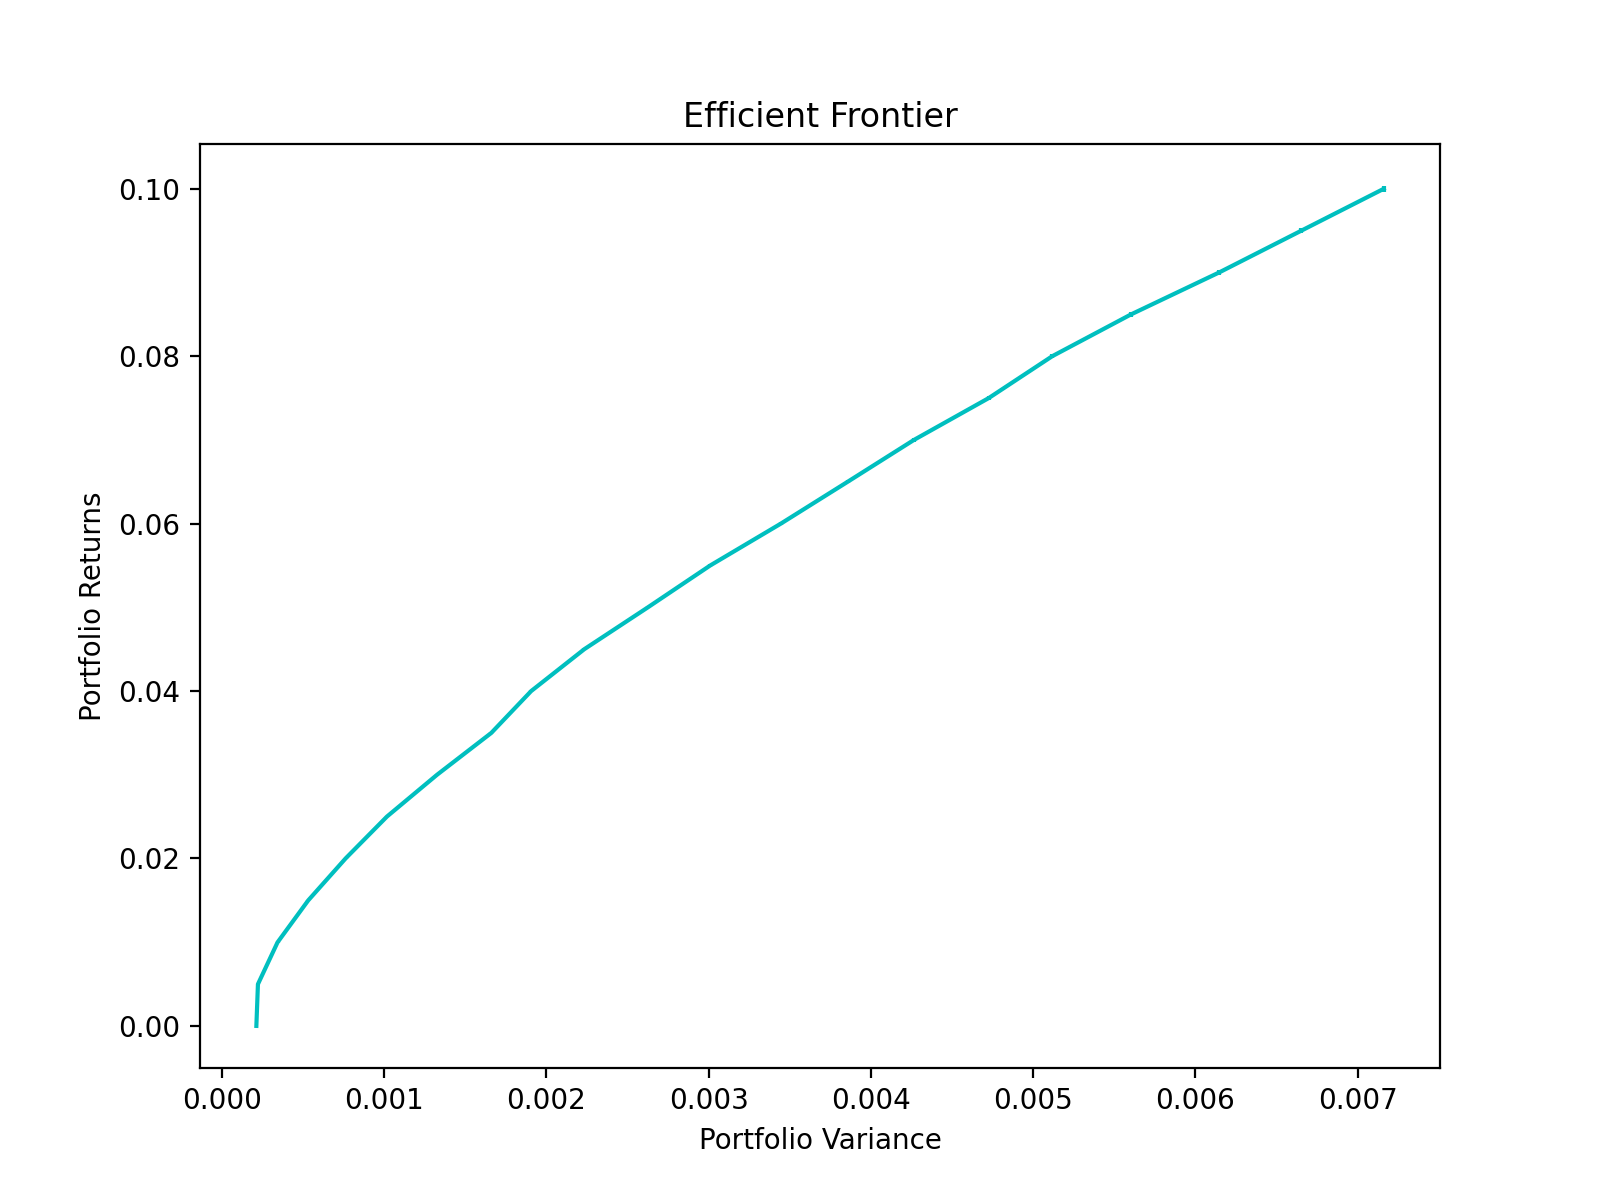
\includegraphics[width=\textwidth]{figures/is_ef.png}}
	\caption{A plot of the efficient frontier marked out by 21 portfolios generated by the application on in sample data. Error bars are included, though are very small. The data is used for them is the portfolio variance.}
	\label{fig:is_ef}
\end{figure}


Encouragingly, in Figures \ref{fig:is_ef} and \ref{fig:oos_ef} we see the correct shape in the efficient frontiers of the portfolio returns and variances generated both in and out of sample in that both are concave in general.

The in sample frontier is particularly promising as it is monotonically increasing with a negative second derivative (or curvature) as required. It echoes the top portion of Figure \ref{fig:efficient_frontier} well.



\begin{figure}[H]
	\centerline{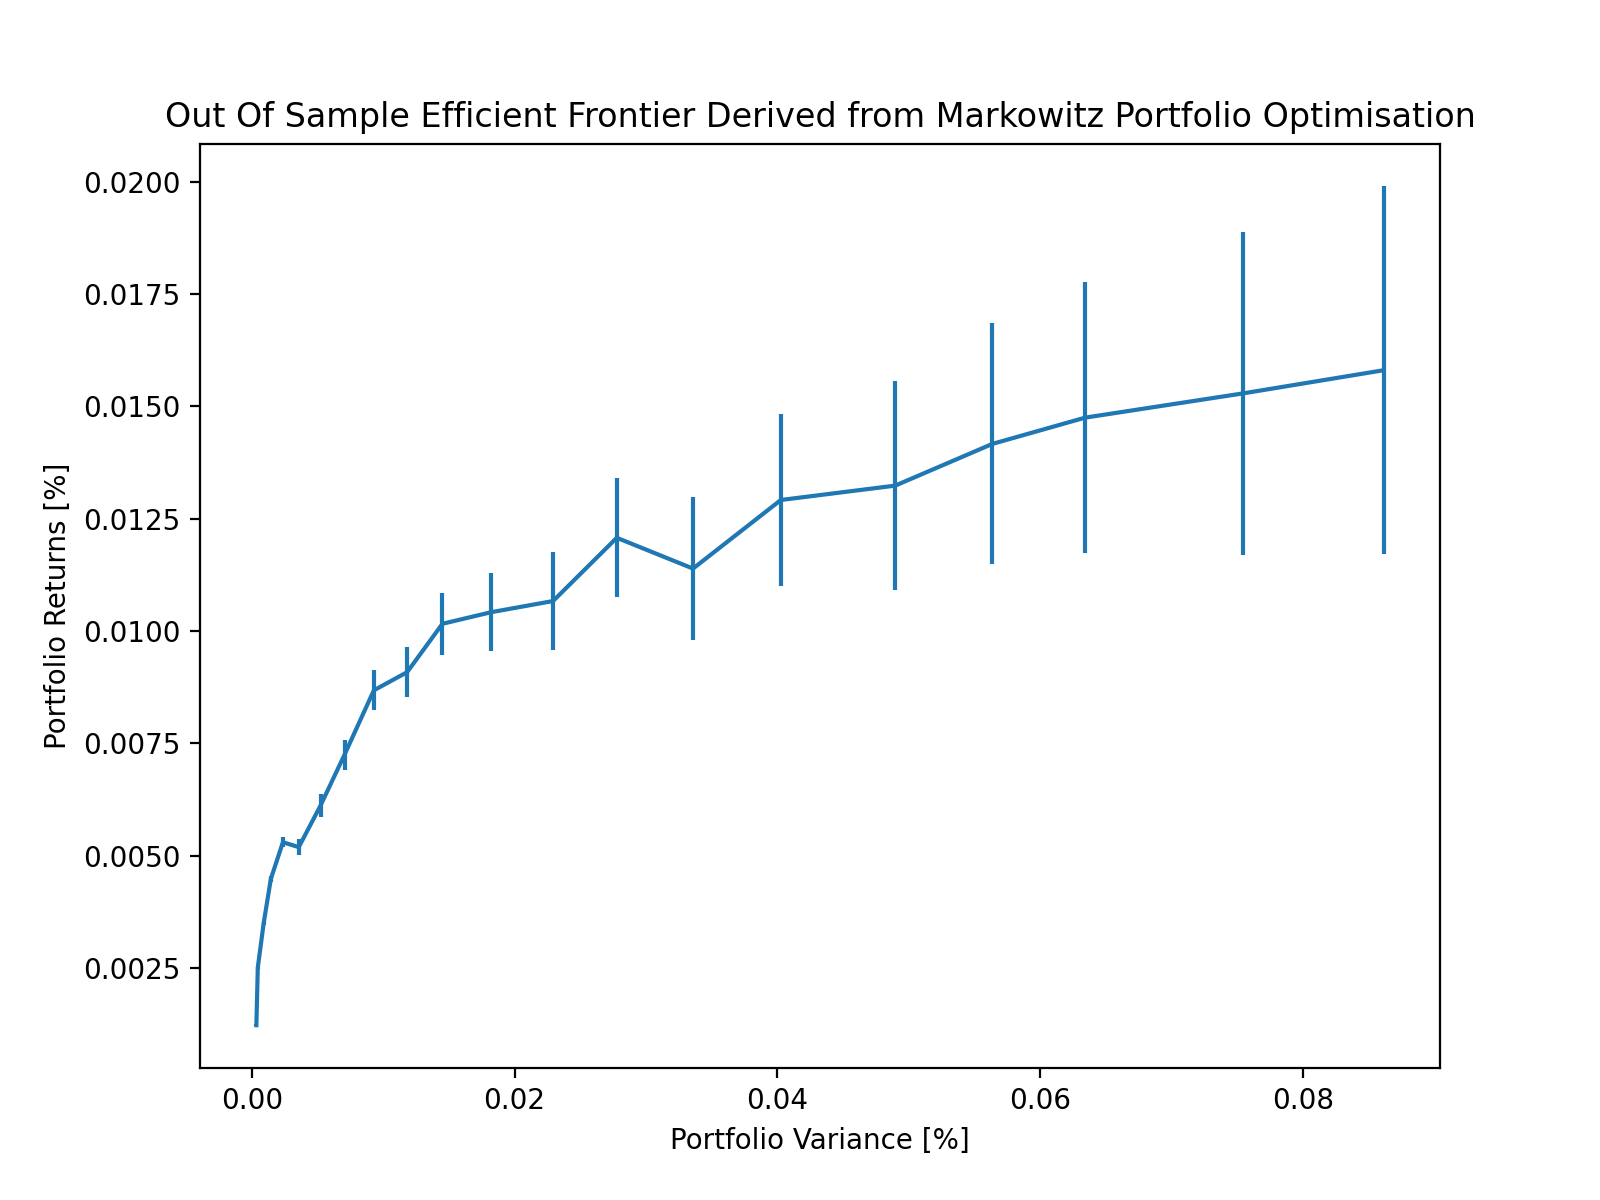
\includegraphics[width=\textwidth]{figures/oos_ef.png}}
	\caption{A plot of the efficient frontier marked out by 21 portfolios generated by the application on out of sample data. Data used for the error bars is the portfolio variance itself.}
		\label{fig:oos_ef}
\end{figure}


The out of sample efficient frontier still yields the correct shape in line with the a fundamental of portfolio choice theory - the more systemic risk taken on by a portfolio, the more heavily they are compensated. 

The data used for the error bars is the variance; employed here to highlight more clearly a subtle phenomenon at play. As the target return is increased, the algorithm "searches" across the dataset of 83 assets over the 100 days of the backtesting window "looking" for more profitable assets to invest in, to meet the higher target. Once a certain target level of return, $\overline{r_p}*$ is required, the pool of assets profitable enough (where $r_i \geq \overline{r_p}*$ for arbitrary asset $i$) \textit{shrinks}. This is to say that the target level of return is scarcely seen in the dataset and so the method is faced with the difficult task of assigning weights such that $\overline{r_p}* = \overline{r_p} = \sum_{i=1}^{n} \overline{r_{i}}w_{i}$ while subject to the constraint that $\sum_{i=1}^{n}w_{i} = 1$ despite $r_i \leq \overline{r_p}*$ for an increasingly large proportion of the $n$ assets available. As a solution, it produces weights ${w_i}$ such that $|w_i| \geq 1$ more frequently and larger in magnitude, translating to larger long positions and equivalently larger short positions (to maintain the fund allocation constraint, Equation (\ref{eqn:weights_constraint})). This in turn, sees the portfolio variance increase quickly in its attempt to meet the target return constraint.

Similarly, it stands to reason that if the portfolio is quickly running out of headroom in terms of profiting when the asset values increase, it must turn to satisfy its constraints by seeking to profit when asset values decrease; the Quadratic Conjugate Method "recommends" short selling more frequently when target returns are higher. Up to a point, the fraction of weigths $w_i \leq 0$ increases with $\overline{r_p}$, until the portfolio cannot satisfy the target return constraint, short selling or not. This is exemplified below in Figure \ref{fig:nShorts} and Table \ref{table:nShorts} of the Appendix.

\begin{figure}[H]
	\centerline{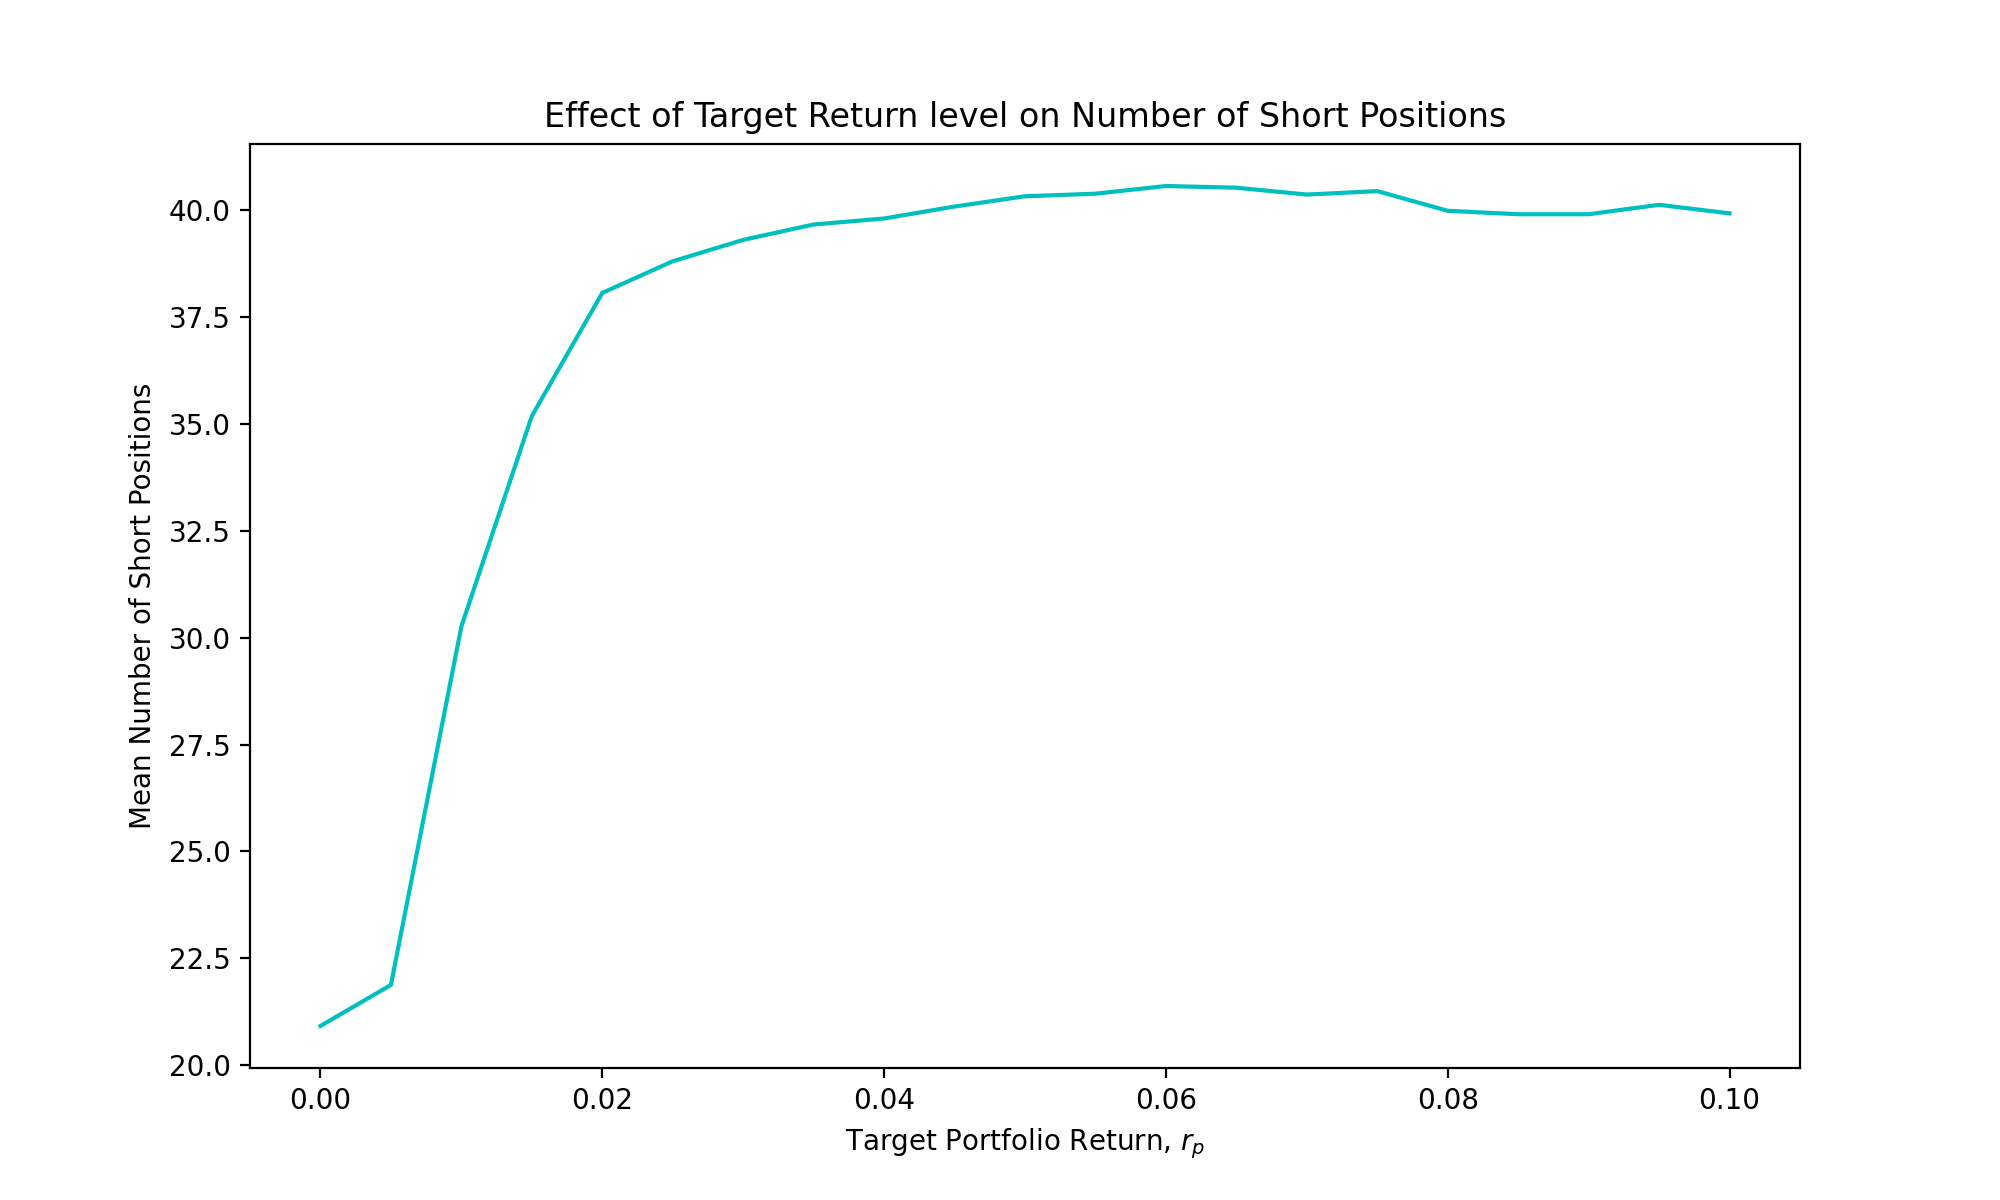
\includegraphics[width=\textwidth]{figures/nShorts.png}}
	\caption{We see the number of short positions taken up increase sharply with the target return set before flattening asymptotically as the system finds that more portfolio return cannot be realised, whether or not the number of short positions is increased further.}
	\label{fig:nShorts}
\end{figure}


As a result of these factors, portfolio volatility increases as the variability in the returns increases since the pool of relatively attractive assets shrinks and positions on those assets are larger in magnitude

This explains the $\approx 48$ fold increase seen in variance across in and out of sample portfolios yielding the same realised return. (See Table \ref{table:port_results}; when the in sample portfolio yielded 1\% in realised returns it held a 0.03\% in sample variance. Similarly for a portfolio to realise 1\% out of sample the target return was in fact 5\% and the corresponding realised variance was 1.45\%.)



The preceding variance discussion above is exemplived in Figure \ref{fig:plot_evolution}. For increasing targets, the realised portfolio returns increase marginally in comparison to the increased risk taken on. 


\begin{figure}[H]
	\centerline{\includegraphics[width=\textwidth]{figures/plot_evolution.png}}
	\caption{The evolution of a subset of the 21 portfolios tested. They are plotted against the evolution of the market as well as the target return and market and portfolio means.}
	\label{fig:plot_evolution}
\end{figure}



\subsection{Performance}

As C++ was chosen as the language, the application's performance from a computational standpoint must be addressed. Running the backtest across the full dataset of 700 days and $n=83$ assets a total of 20 times for each target return, the mean and standard error were calculated. The result was $14598.6 \pm 10.5\;ms$. \footnote{Note that this was achieved on Linux machine with an i7-3770K CPU overclocked to 4.8GHz across all 4 cores and so reproducability in the exact figures mentioned here may not be possible. Despite this, the order of complexity of the application will remain unchanged.}

Furthermore, the time complexity of the application was computed as a function of the number of assets in the dataset considered. Figure \ref{fig:time_complexity_in_assets} below shows the increase in time taken to run one complete simulation, with the number of assets considered. Each simulation looped over all 700 days for each of the 21 target returns from 0\% to 10\% in 0.5\% increments with the number of assets considered the exogenous variable.

One would expect the time complexity in asset number to be of second order given that the most intensive arithmetic operation required is iterating over the rows and columns of a covariance matrix, an $\mathcal{O}(n^2)$ operation. In the implementation of the optimisation method above, the matrix $A \in \Re^{(n+2) \times (n+2)}$, containing the covariance matrix $\Sigma \in \Re^{n \times n} $ for $n$ assets was iterated over. However, despite the aforementioned efficient implementation of \textit{ParameterEstimator::estimateCovariances()} capitalising on the symmetry property of the covariance matrix, (as can be seen in section \ref{sec:parameter_estimation}), it was found that the time complexity of the application remains as $\mathcal{O}(n^2)$ in the number of assets, $n$.


In Figure \ref{fig:time_complexity_in_assets} we see an increasing relation between assets and time complexity, to which linear, quadratic and cubic polynomials were fitted. The quadratic polynomial yielded the fit with the lowest mean squared error, closer to the actual curve than the cubic by a thin margin.

The difference between them was small enough to warrant that more datapoints at larger values of asset number are required in order to discern between the two irrefutably.

\begin{figure}[H]
	\centerline{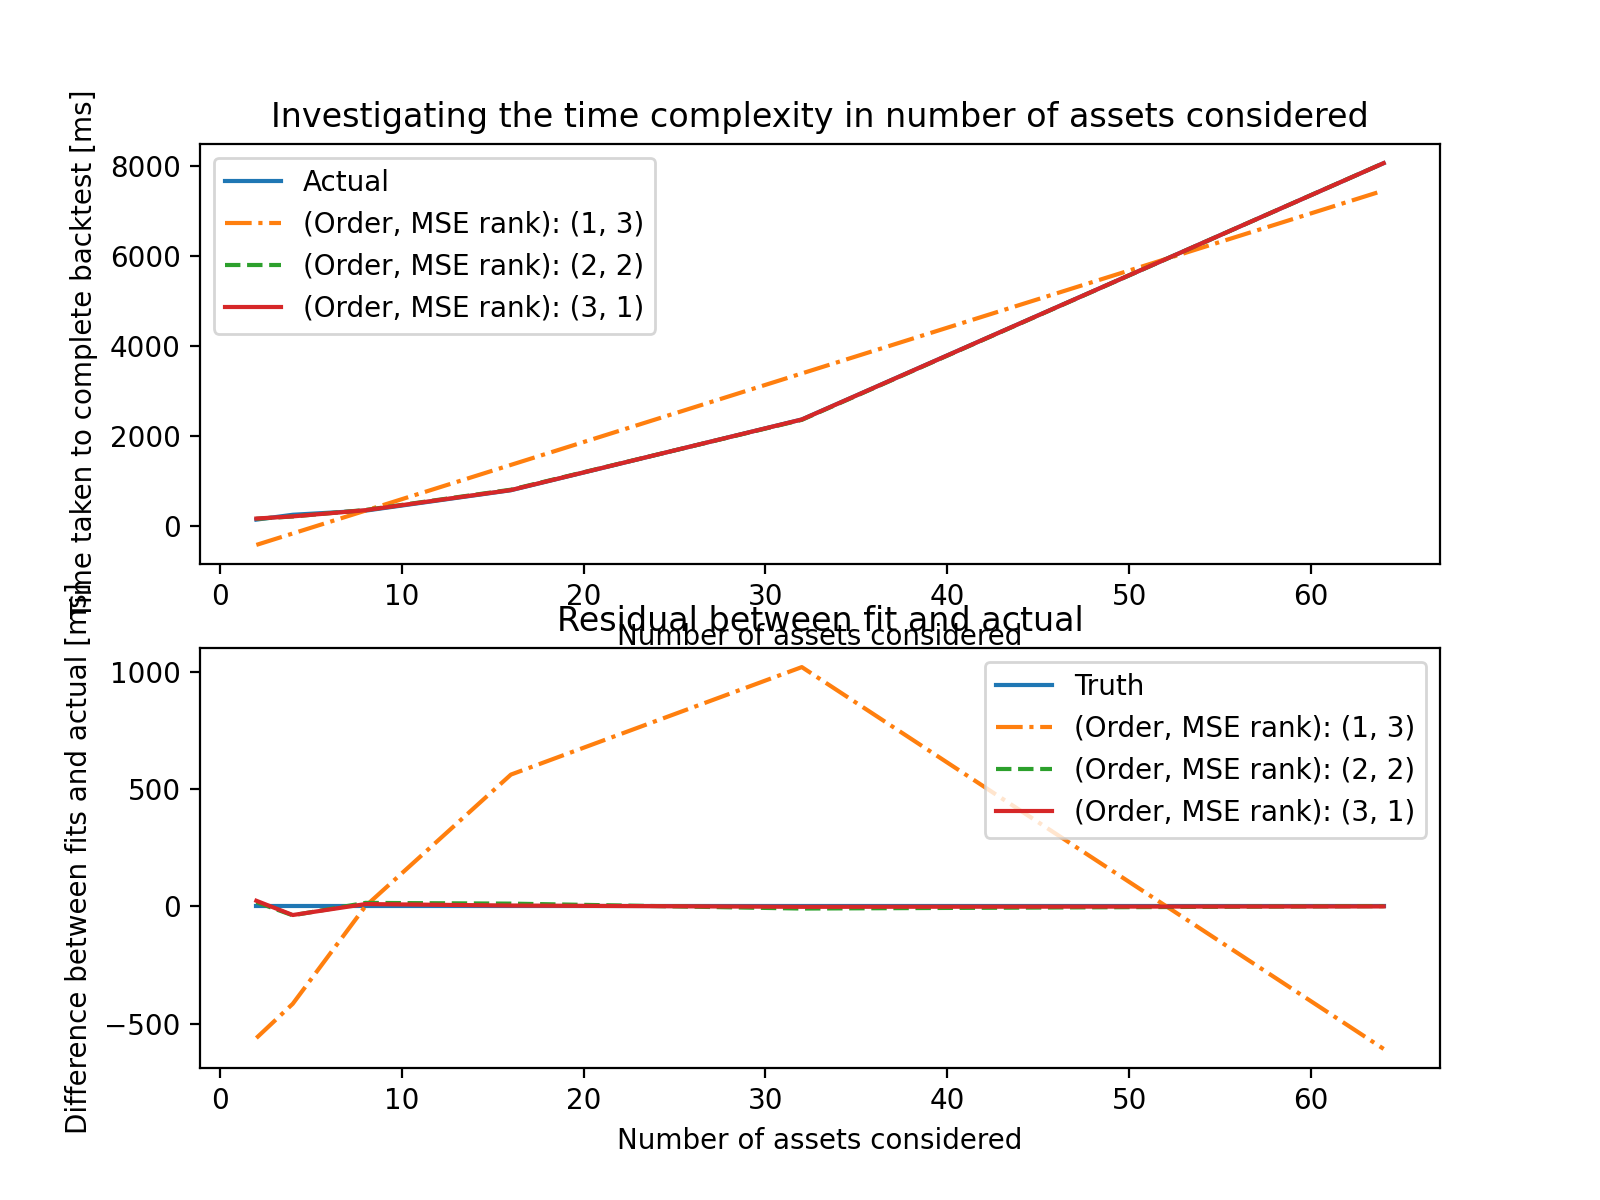
\includegraphics[width=\textwidth]{figures/time_complexity_in_assets.png}}
	\caption{Time complexity of the application as a function of number of assets considered. Linear, quadratic and cubic polynomials were fitted and their rank order in terms of MSE shown in the legends, with a rank of 1 assigned to the fit with the lowest mean squared error. The coefficients $a$, $b$ and $c$ for the prevailing quadratic of the form $a* assets^2 + b * assets + c$ were: 3.358 $ms/asset^{2}$, 18.0897 $ms/asset$ and 143.660 $ms$.}
	\label{fig:time_complexity_in_assets}
\end{figure}



\section{Conclusions}
\label{sec:concs}


This investigation was successful in its implementation of the Quadratic Conjugate Method, displayed thoroughly by the adherance of the in sample results to the theoretical results and constraints imposed.

It was also instrumental in offering a means to delve deeper into aspects of the Markowitz portfolio choice approach beyond a surface level. It was shown in the preceding sections that the shortcomings of the application's ability to produce a portfolio yielding the specified target return was not a failing of its implementation, but rather a failing of the assumptions behind Markowitz Portfolio Theory.

Nevertheless, results such as the portfolios' evolution over the testing periods and their efficient frontiers all corroborated with what was expected according to portfolio choice theory.

Insightful extensions to this investigation may include the implementation of a naive model, assigning weights from a random uniform distribution and comparing the performance both financially and computationally of this portfolio to the Markowitz one. This may provide a sound benchmark for the Markowitz approach to be compared to.

Useful results drawn from the application having ingested a non-trivial dataset in a performant manner, is further testament to the commendable, mathematically proven horizon of convergence of the Quadratic Conjugate Method, and this implementation in C++.



\newpage

\begin{thebibliography}{}
\label{sec:thebibliography}
	\bibitem{ef_medium} Medium. 2020. Fábio Neves. [ONLINE] Available at: https://towardsdatascience.com/python-markowitz-optimization-b5e1623060f5. [Accessed 8 June 2020].
	\bibitem{capm} Black, Fischer., Michael C. Jensen, and Myron Scholes (1972). The Capital Asset Pricing Model: Some Empirical Tests, pp. 79–121 in M. Jensen ed., Studies in the Theory of Capital Markets. New York: Praeger Publishers.
	\bibitem{mpt} Markowitz, H.M. (March 1952). "Portfolio Selection". The Journal of Finance. 7 (1): 77–91. doi:10.2307/2975974. JSTOR 2975974.
	\bibitem{notes} Parpas, P. "Computational Finance with C++, Numerical Methods for Optimization Models" pp. 27-37, Imperial College London
	\bibitem{assignment} Parpas, P. "Computational Finance with C++, Coursework 2020" pp. 2, Imperial College London
	\bibitem{qcm_convergence} Saad, Yousef (2003). Iterative methods for sparse linear systems (2nd ed.). Philadelphia, Pa.: Society for Industrial and Applied Mathematics. pp. 195. ISBN 978-0-89871-534-7.
	\bibitem{martingale} Thomas Delcey. Samuelson vs Fama on the Efficient Market Hypothesis: The Point of View of Expertise. Œconomia - History/Methodology/Philosophy, NecPlus/Association Œconomia, 2019, Varia,
	9 (1), pp.37-58. ffhal-01618347v2f
	
	
	
\end{thebibliography} 



\section{Appendix} 
\label{sec:appendix}

\subsection{Additional Figures} 
\label{sec:add_figs}

\begin{center}
	\begin{table}[H]
\begin{tabular}{|c c c c c|} 
			\hline
			Target Return [\%] & IS Return  [\%]&	 IS Var [\%]  & OOS Return [\%]  & OOS Var [\%]  \\ [0.5ex] \hline \hline
			0.00  	 &	-0.00031  &	0.021275  	 &	0.12256  &	0.03516	\\ \hline
			0.50	 &	0.49835	  &	0.022244	 &	0.25074  &	0.04595	\\ \hline
			1.00	 &	0.99761   &	0.034314  	 &	0.34959  &	0.09076	\\ \hline
			1.50	 &	1.49924	  &	0.053232  	 &	0.44820  &	0.14525	\\ \hline
			2.00	 &	2.00077	  &	0.076287  	 &	0.53001  &	0.23714	\\ \hline
			2.50	 &	2.50061	  &	0.101759	 &	0.51905  &	0.35774		\\ \hline
			3.00	 &	3.00013	  &	0.132648	 &	0.61174  &	0.52358		\\ \hline
			3.50	 &	3.49999	  &	0.166081	 &	0.72476  &	0.70585		\\ \hline
			4.00	 &	4.00003	  &	0.190654	 &	0.86816  &	0.92924		\\ \hline
			4.50	 &	4.49993	  &	0.223382	 &	0.90854  &	1.18221		\\ \hline
			5.00	 &	4.99995	  &	0.262566	 &	1.01628	 &	1.45095		\\ \hline
			5.50	 &	5.50003	  &	0.300989	 &	1.04214	 &	1.82303		\\ \hline
			6.00	 &	6.00000	  &	0.344525	 &	1.06694	 &	2.29281		\\ \hline
			6.50	 &	6.50003	  &	0.385709	 &	1.20770	 &	2.77746		\\ \hline
			7.00	 &	7.00002	  &	0.426567	 &	1.13917	 &	3.35760		\\ \hline
			7.50	 &	7.49995	  &	0.472654	 &	1.29186	 &	4.02585		\\ \hline
			8.00	 &	8.00025	  &	0.511818	 &	1.32384	 &	4.89597		\\ \hline
			8.50 	 &	8.50035	  &	0.560443	 &	1.41675	 &	5.63572		\\ \hline
			9.00	 &	9.00035	  &	0.614633	 &	1.47520	 &	6.34150		\\ \hline
			9.50	 &	9.50042	  &	0.665383	 &	1.52919	 &	7.54353		\\ \hline
			10.0 	 &	9.99979	  &	0.716094	 &	1.58072	 &	8.61231 \\ [1ex]  \hline


\end{tabular}
\caption{Output from a run of the application for daily target returns from 0\% to 10\% in 0.5\% steps.}
\label{table:port_results}
	\end{table}
\end{center}


\begin{center}{
	\begin{table}[H]
		\centering
		\begin{tabular}{|c c |} 
			\hline
			Target Return [\%] & nShorts \\ [0.5ex] \hline \hline
					0.00	& 20.92 \\ \hline
					0.50 	& 21.88 \\ \hline
					1.00 	& 30.26 \\ \hline
					1.50	 & 35.18 \\ \hline
					2.00 	& 38.06 \\ \hline
					2.50 	& 38.8 \\ \hline
					3.00 	& 39.3 \\ \hline
					3.50 	& 39.66 \\ \hline
					4.00 	& 39.8 \\ \hline
					4.50	 & 40.08 \\ \hline
					5.00	& 40.32 \\ \hline
					5.50 	& 40.38 \\ \hline
					6.00 	& 40.56 \\ \hline
					6.50 	& 40.52 \\ \hline
					7.00 	& 40.36 \\ \hline
					7.50 	& 40.44 \\ \hline
					8.00	& 39.98 \\ \hline
					8.50 	& 39.9 \\ \hline
					9.00	& 39.9 \\ \hline
					9.50 	& 40.12 \\ \hline
					10.00	& 39.92 \\ [1ex] \hline
		\end{tabular}
		\caption{nShorts is the mean average number of short positions reccomended by the quadratic conjuaget method and then subsequently opened by the portfolio.}
		\label{table:nShorts}
	\end{table}
}
\end{center}

\begin{center}{
\begin{table}[H]
	\centering
\begin{tabular}{|c c|} 
\hline
Run & Time Taken [ms]  \\ [0.5ex] 
\hline\hline
1 & 14760 \\
\hline
2 & 14519 \\
\hline
3 & 14557 \\
\hline
4 & 14569 \\
\hline
5 & 14551 \\
\hline
6 & 14575 \\
\hline
7 & 14593 \\
\hline
8 & 14601 \\
\hline
9 & 14598 \\
\hline
10 & 14594 \\
\hline
11 & 14588 \\
\hline
12 & 14620 \\
\hline
13 & 14582 \\
\hline
14 & 14602 \\
\hline
15 & 14591 \\
\hline
16 & 14600 \\
\hline
17 & 14609 \\
\hline
18 & 14607 \\
\hline
19 & 14610 \\
\hline
20 & 14646 \\ [1ex] 
20 & 14646 \\ [1ex] 
\hline
\end{tabular}
\caption{The time taken for full runs of the backtesting application over all 83 assets and 700 days. \textbf{Mean} $\pm$ \textbf{ standard error: } $14598.6 \pm 10.5\;ms$}
\label{table:timings}
\end{table}
}
\end{center}

\subsection{Code} 
\label{sec:code}

All code found below is also stored in the public repository for your convenience:

\href{https://github.com/indipanesar96/markowitzportfoliooptimiser.git}{https://github.com/indipanesar96/markowitzportfoliooptimiser.git}


\end{document}